\documentclass[tikz,border=2pt]{standalone}
\usepackage{amsmath}
\usepackage{pgfplots}
\pgfplotsset{compat=1.18}
\usetikzlibrary{arrows.meta}
\begin{document}
% Example 6.1: [A,I_3] for x1<=4, 2x2<=12, 3x1+2x2<=18; basis {3,2,1} in the order (x3,x2,x1) picks the columns
% A3,A2,A1 into B, B^{-1}b=(2,6,2) is the corner (2,6) where x4=0 and x5=0 are binding;
% other bases: {3,4,5} -> (0,0), {3,2,5} -> (0,6), {1,2,5} -> (4,6) infeasible (x5=-6).
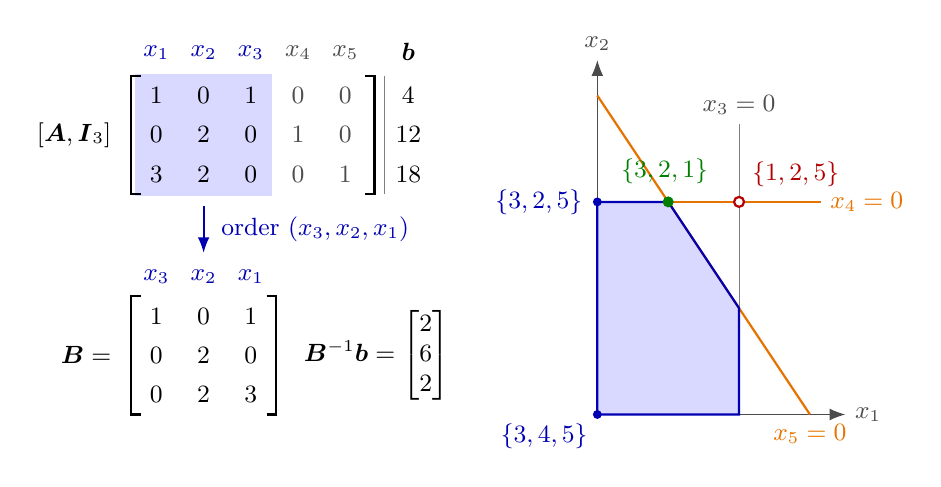
\begin{tikzpicture}[font=\small, >={Latex[length=2mm]}]
  % ---------- left: the columns of [A, I_3] ----------
  \begin{scope}
    \fill[blue!15] (-0.27,-0.28) rectangle (1.47,-1.82);
    \foreach \j/\x in {1/0,2/0.6,3/1.2} \node[blue!70!black] at (\x,0) {$x_{\j}$};
    \foreach \j/\x in {4/1.8,5/2.4} \node[gray!60!black] at (\x,0) {$x_{\j}$};
    \node at (3.2,0) {$\boldsymbol{b}$};
    \foreach \r/\y/\a/\bb/\c/\d/\e/\f in {1/-0.55/1/0/1/0/0/4, 2/-1.05/0/2/0/1/0/12, 3/-1.55/3/2/0/0/1/18} {
      \node at (0,\y) {$\a$}; \node at (0.6,\y) {$\bb$}; \node at (1.2,\y) {$\c$};
      \node[gray!60!black] at (1.8,\y) {$\d$}; \node[gray!60!black] at (2.4,\y) {$\e$};
      \node at (3.2,\y) {$\f$};
    }
    \draw[thick] (-0.2,-0.3) -- (-0.32,-0.3) -- (-0.32,-1.8) -- (-0.2,-1.8);
    \draw[thick] (2.65,-0.3) -- (2.77,-0.3) -- (2.77,-1.8) -- (2.65,-1.8);
    \draw[gray] (2.9,-0.3) -- (2.9,-1.8);
    \node[anchor=east] at (-0.45,-1.05) {$[\boldsymbol{A},\boldsymbol{I}_{3}]$};
    % arrow down to B
    \draw[->, blue!70!black, thick] (0.6,-1.95) -- (0.6,-2.55);
    \node[blue!70!black, anchor=west] at (0.7,-2.25) {order $(x_3,x_2,x_1)$};
    % B
    \foreach \j/\x in {3/0,2/0.6,1/1.2} \node[blue!70!black] at (\x,-2.85) {$x_{\j}$};
    \foreach \y/\a/\bb/\c in {-3.35/1/0/1, -3.85/0/2/0, -4.35/0/2/3} {
      \node at (0,\y) {$\a$}; \node at (0.6,\y) {$\bb$}; \node at (1.2,\y) {$\c$};
    }
    \draw[thick] (-0.2,-3.1) -- (-0.32,-3.1) -- (-0.32,-4.6) -- (-0.2,-4.6);
    \draw[thick] (1.4,-3.1) -- (1.52,-3.1) -- (1.52,-4.6) -- (1.4,-4.6);
    \node[anchor=east] at (-0.45,-3.85) {$\boldsymbol{B}=$};
    \node[anchor=west] at (1.75,-3.85) {$\boldsymbol{B}^{-1}\boldsymbol{b}=\begin{bmatrix}2\\6\\2\end{bmatrix}$};
  \end{scope}
  % ---------- right: the basic solutions as points ----------
  \begin{scope}[shift={(5.6,-4.6)}, x=0.45cm, y=0.45cm]
    \fill[blue!15] (0,0) -- (4,0) -- (4,3) -- (2,6) -- (0,6) -- cycle;
    \draw[gray!60, thin] (0,0) -- (6.6,0) (0,0) -- (0,9.6);
    \draw[->, gray!60!black] (0,0) -- (7,0) node[anchor=west] {$x_1$};
    \draw[->, gray!60!black] (0,0) -- (0,10) node[anchor=south] {$x_2$};
    \draw[gray, thin] (4,0) -- (4,8.2);
    \node[gray!60!black, anchor=south] at (4,8.2) {$x_3=0$};
    \draw[orange!90!black, thick] (0,6) -- (6.3,6);
    \node[orange!90!black, anchor=west] at (6.3,6) {$x_4=0$};
    \draw[orange!90!black, thick] (0,9) -- (6,0);
    \node[orange!90!black, anchor=north] at (6,0) {$x_5=0$};
    \draw[blue!70!black, thick] (0,0) -- (4,0) -- (4,3) -- (2,6) -- (0,6) -- cycle;
    \fill[blue!70!black] (0,0) circle (1.6pt) (0,6) circle (1.6pt);
    \fill[green!50!black] (2,6) circle (2pt);
    \draw[red!70!black, thick, fill=white] (4,6) circle (1.8pt);
    \node[blue!70!black, anchor=north east] at (0,0) {$\{3,4,5\}$};
    \node[blue!70!black, anchor=east] at (-0.15,6) {$\{3,2,5\}$};
    \node[green!50!black, anchor=south] at (1.9,6.25) {$\{3,2,1\}$};
    \node[red!70!black, anchor=south west] at (4.1,6.15) {$\{1,2,5\}$};
  \end{scope}
\end{tikzpicture}
\end{document}
